\section{Principles \& Strategy}
\subsection{Uneven Potential}
Due to how cubes need to be rotated before they are moved, some positions are more dangerous to you than others. A low cube is always in danger of being pinched by the next higher cube if situated an odd number of spaces away. Similarly a high cube is in danger from the next lower cube an even number of spaces away.

Because of this, you will likely find yourself in a situation where the safest course of action is either to not move at all, or to see if you can land far enough away to be out of reach by any cube that is one rotation away from capturing it.

Same-valued cubes are never in any danger, but also never pose a threat.
\subsection{Universal Reachability}
After having played the game a few times, you may start to notice an interesting pattern arising:
\begin{itemize}
    \item Any cube an even number of spaces away, can always be reached by a higher even number.
    \item Any cube an odd number of spaces away, can always be reached by a higher odd number.
\end{itemize}
In other words, if a cube you wish to Pinch or form a Set with is one space away, then it is always reachable with a \epsdice{1}, \epsdice{3}, or \epsdice{5}.
Similarly, a cube two spaces away can always be reached with a \epsdice{2}, \epsdice{4}, or \epsdice{6}.

Due to the movement rule that states cubes cannot cross the same space twice, you can always be certain that if the shortest path is even, no odd roll will ever reach the target square.

This universal reachability principle is also what makes the \textit{Uneven Potential} so dangerous.
Unless you make sure to stay \textit{enough} spaces away, any high enough roll of a given evenness will be able to reach the cube you are trying to protect.
With a board only $5\times 5$ spaces in size, finding a place to hide may be a challenge.

Figure~\ref{fig:odd-reachability} shows how you can reach the same space with every type of odd roll, simply due to the fact that it is one space away. It is easy to see, how with an even move, you would always be a move short or a move too far from the target, hence only odd moves can reach odd spaces and vice versa.
\begin{figure}
    \centering
    \begin{minipage}{0.3\textwidth}
        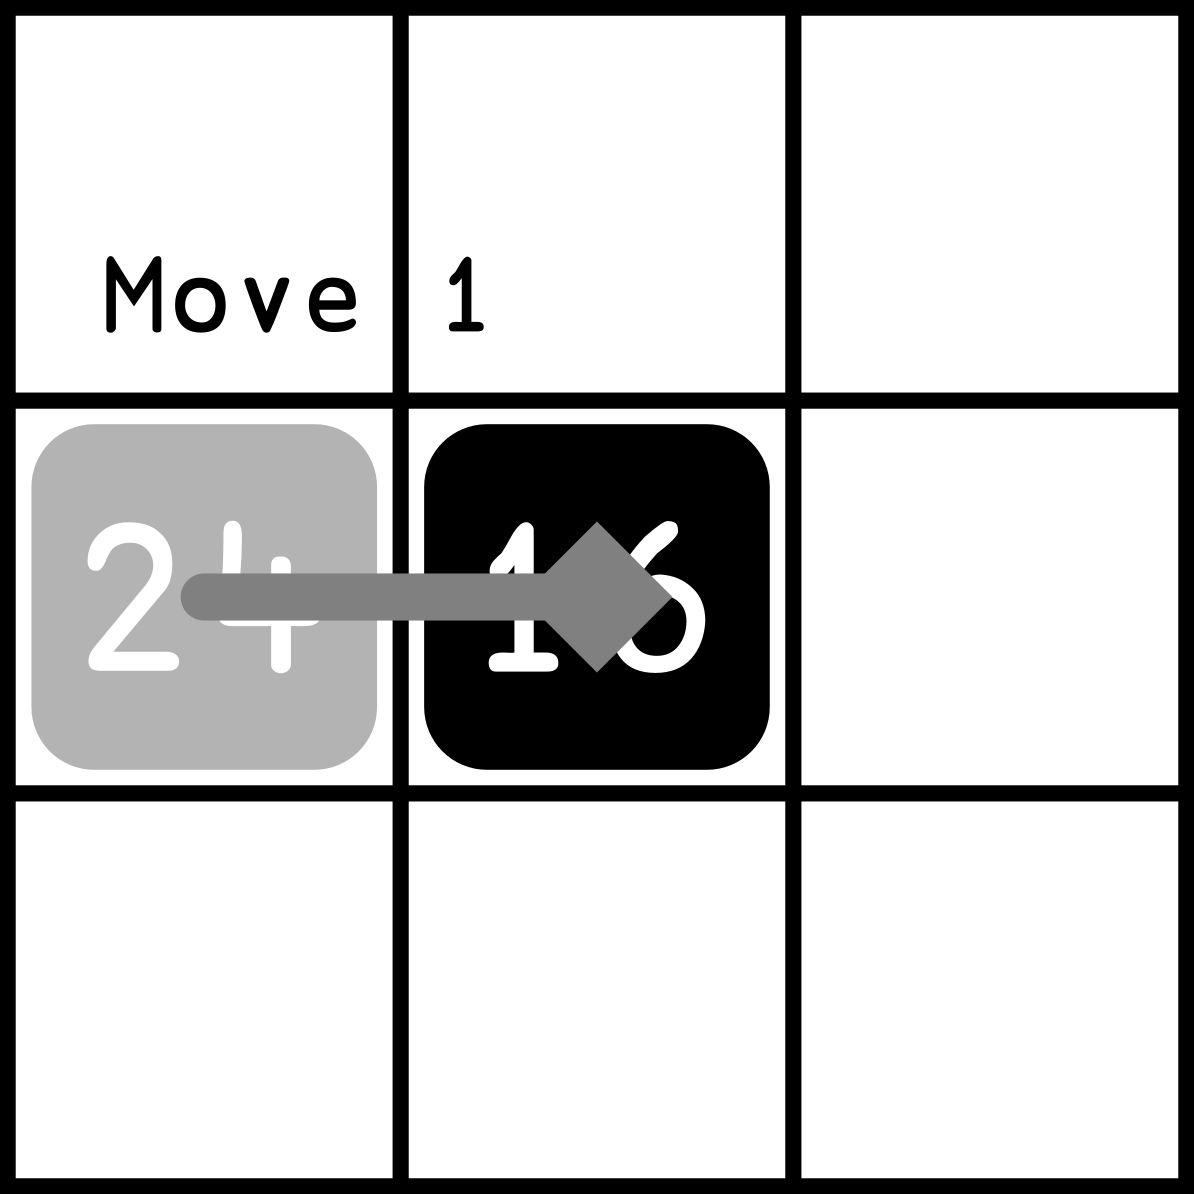
\includegraphics[width=\textwidth]{../graphics/move-1}
    \end{minipage}
    \begin{minipage}{0.3\textwidth}
        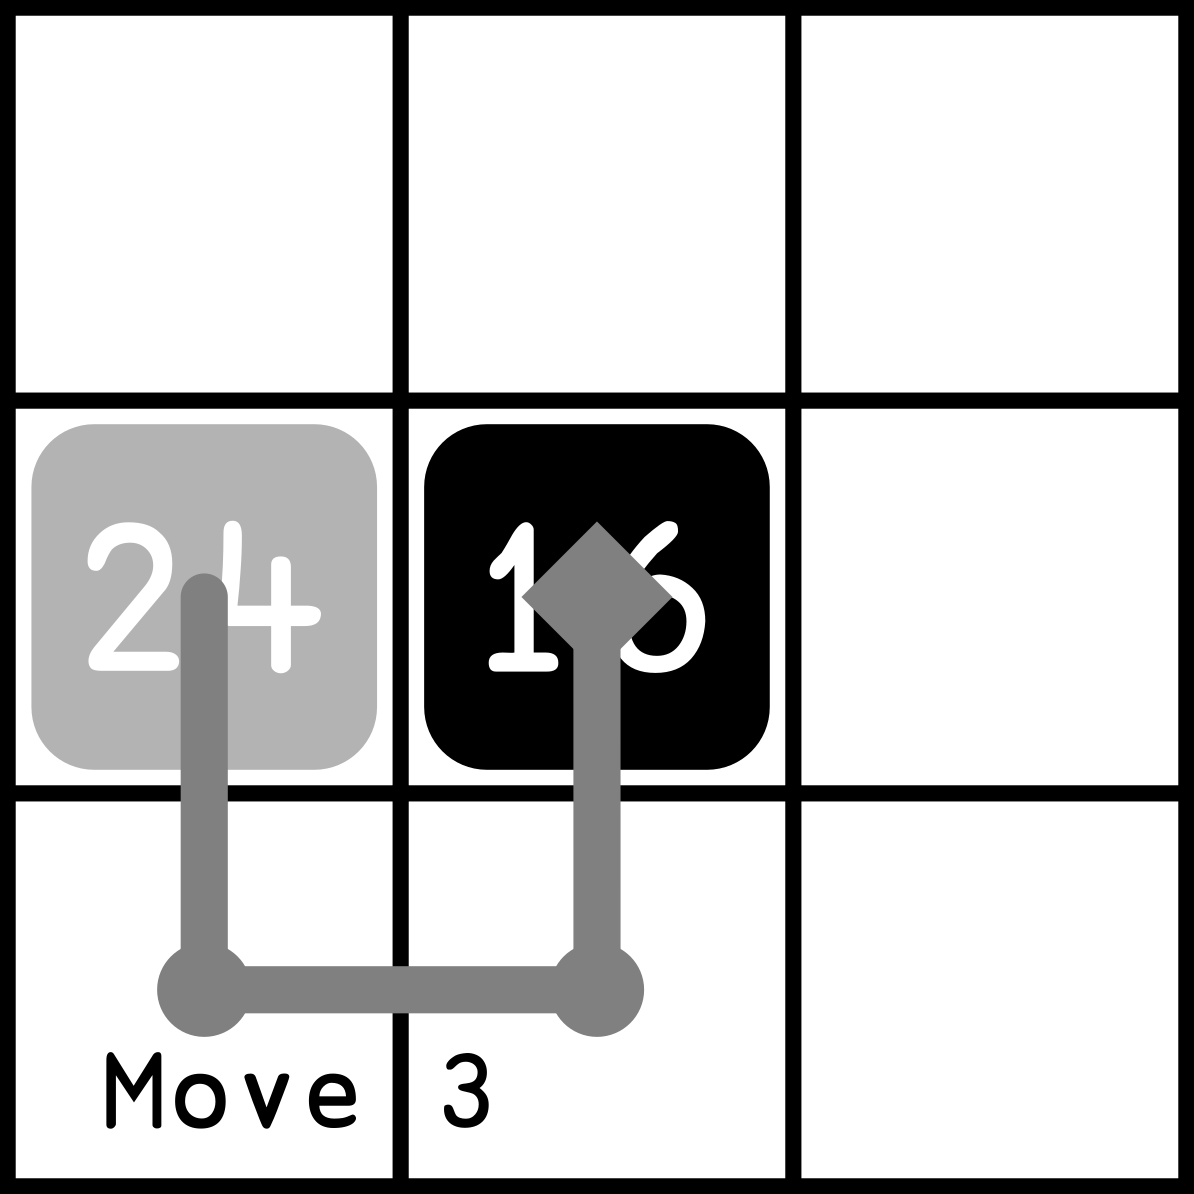
\includegraphics[width=\textwidth]{../graphics/move-3}
    \end{minipage}
    \begin{minipage}{0.3\textwidth}
        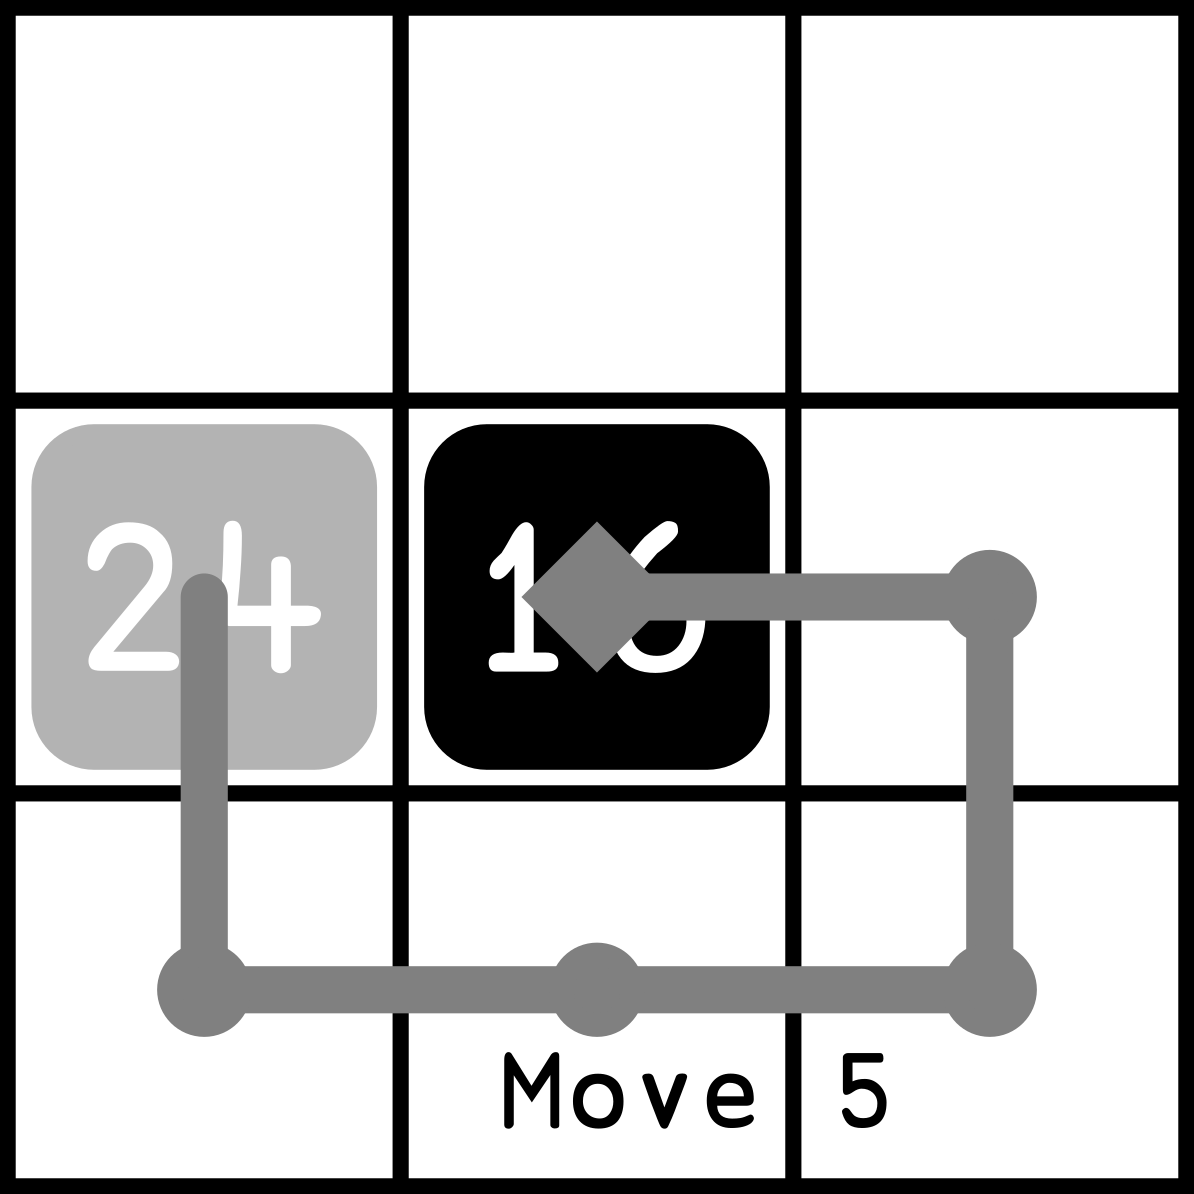
\includegraphics[width=\textwidth]{../graphics/move-5}
    \end{minipage}
    \caption{A spot an uneven number of spaces away}
    \label{fig:odd-reachability}
\end{figure}